\documentclass{article}%
\usepackage[T1]{fontenc}%
\usepackage[utf8]{inputenc}%
\usepackage{lmodern}%
\usepackage{textcomp}%
\usepackage{lastpage}%
\usepackage{authblk}%
\usepackage{graphicx}%
%
\title{LRP{-}6 is a coreceptor for multiple fibrogenic signaling pathways in pericytes and myofibroblasts that are inhibited by DKK{-}1}%
\author{Angela Decker}%
\affil{Institute of Bioinformatics and Biosignal Transduction, College of Bioscience and Biotechnology, National Cheng{-}Kung University, Tainan, Taiwan}%
\date{01{-}01{-}2013}%
%
\begin{document}%
\normalsize%
\maketitle%
\section{Abstract}%
\label{sec:Abstract}%
SAN DIEGO (KSNT){-} You may have heard recently about the evolution of a novel regulatory treatment for colon cancer. The therapy, called K{-}RAS{-}dependent migration, or KRAM, is designed to inhibit DNA replication{-}dependent metastasis to the GI tract and enhance adherence to chemotherapy and other chemotherapy agents.\newline%
That kind of activity, said Dan Pirro{-} Wechsler, a professor of urology and Radiation Oncology at the UC San Diego School of Medicine and assistant director of Cancer Translational Biology at MD Anderson Cancer Center.\newline%
This regulatory regulation, KRAM, is incredibly efficient in allowing the local replication of its target to cause apoptosis. Furthermore, it avoids the consequences of tumor cell death in the same way that tumor cells may own calcium signaling channel CGC, which is activated by DNA replication.\newline%
Tumor cells are also initially activating drugs when they are activated by replication of KRAM. This trigger mechanism eventually enables the replication of mutant colon tumor cells so that the patients tumor cells will multiply in increased numbers, said Pirro{-}Wechsler.\newline%
KRAM is still a study and there is ongoing need for more research and refinement in his lab, however, Its happening as a result of constant high level cultivation for this type of work by our highly skilled group of scientists, said Pirro{-}Wechsler.

%
\subsection{Image Analysis}%
\label{subsec:ImageAnalysis}%


\begin{figure}[h!]%
\centering%
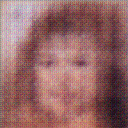
\includegraphics[width=150px]{500_fake_images/samples_5_199.png}%
\caption{A Man With A Beard Wearing A Tie And Glasses}%
\end{figure}

%
\end{document}